\documentclass{beamer}
%
% Choose how your presentation looks.
%
% For more themes, color themes and font themes, see:
% http://deic.uab.es/~iblanes/beamer_gallery/index_by_theme.html
%
\mode<presentation>
{
	\usetheme{Madrid}
  %\usetheme{default}      % or try Darmstadt, Madrid, Warsaw, ...
  \usecolortheme{default} % or try albatross, beaver, crane, ...
  \usefonttheme{default}  % or try serif, structurebold, ...
  \setbeamertemplate{navigation symbols}{}
  \setbeamertemplate{caption}[numbered]
} 

\usepackage[english]{babel}
\usepackage[utf8x]{inputenc}
\usepackage{textcomp}
\usepackage{caption}
\usepackage[bottom]{footmisc}
\usepackage{amsmath}
\usepackage{amsfonts}
\usepackage{amssymb}
\usepackage{amsthm}
\usepackage{mathrsfs}
\usepackage{mathptm}
\usepackage{physics}
\usepackage{times}
\newtheorem{lem}{Lemma}[section]
\newtheorem{theo}[lem]{Theorem}
\newtheorem{defi}[lem]{Definition}
\newtheorem{megall}[lem]{Megállapodás}
\newtheorem{allitas}[lem]{Proposition}
\newtheorem{atfog}[lem]{Átfogalmazás}
\DeclareMathOperator{\dom}{dom}
\DeclareMathOperator{\ess}{ess}
\DeclareMathOperator*{\ch}{ch}

\title[Final Seminar]{On the list coloring of 1-band buffering graphs}
\author{Marine Collery, Benjamin Martin Seregi}
\institute{KTH Royal Institute of Technology\\
II2202, Fall 2017, Period 1-2}
\date{12/01/2018}

\begin{document}

\begin{frame}
  \titlepage
\end{frame}

% Uncomment these lines for an automatically generated outline.
%\begin{frame}{Outline}
%  \tableofcontents
%\end{frame}
%------------------------------------------------
\section{Introduction}

\begin{frame}{Problem Statement}

\justifying
\begin{itemize}
\item A graph $G$ is cellular if it is constructed from a hexagonal cellular topology and
\pause \item we say that it is $1$-band buffering if the interference extends up to $1$ cell.
\end{itemize}
\pause \begin{defi}[$k$-choosability and $k$-list coloring]
Let $G$ be a graph and $L(v)$ a set of colors for all $v \in V(G)$ such that $|L(v)|=k$. We say that $G$ is $k$\textit{-choosable} if $G$ is colorable such that the color of $v$ is in $L(v)$ for all $v \in V(G)$, such colorings called $k$\textit{-list coloring} of $G$.
\pause
\end{defi}
\textbf{Problem:} How to color a graph from the lists $L(v)?$
\end{frame}

%------------------------------------------------
\begin{frame}
\frametitle{Why is it important to study this?}
\justifying
\begin{itemize}
\item A $k$-list coloring of a cellular graph corresponds to an interference-free channel allocation where $L(v)$ is the list of free channels for the access point $v$.
\pause \item Finding the optimal channel allocation is of great interest: with interference-free allocations it is possible to achieve higher throughput.
\pause \item Channel allocation problem is $\mathrm{NP}$-complete in general.
\end{itemize}
\begin{figure}
\caption{3-coloring of a cellular graph, $L(v):=\lbrace \text{PURPLE,YELLOW,BLUE} \rbrace.$}
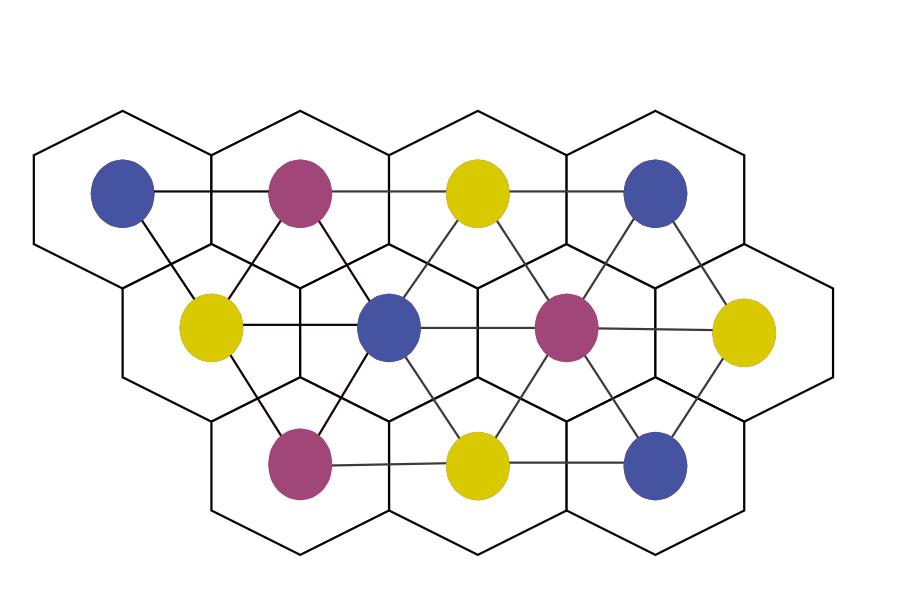
\includegraphics[scale=0.15]{3_coloring_cellular.png}
\end{figure}
\end{frame}

\begin{frame}
\frametitle{Research questions}
\justifying
\begin{itemize}
\item What is the smallest $k > 0$ such that a cellular graph is $k$-choosable (i.e. what is the choice number of cellular graphs)?
\pause \item How can we find an orientation in $G$ such that it is acyclic and $d^+(v) \leqslant 3$ for all $v \in V(G)$ in polynomial time of the size of $G$?
\pause \item Does there exist a polynomial time algorithm that finds a kernel in the previously constructed graph?

\end{itemize}
\end{frame}

\begin{frame}
\frametitle{Answers}
\justifying
\begin{itemize}
\item If $G$ is cellular then $\ch(G) \leqslant 4$ (see Report,  Theorem 2.)
\pause \item It is possible to construct a $3$-bounded acyclic orientation in polynomial time (see Report, Algorithm 1).
\pause \item It is possible to find a kernel in a $3$-bounded acyclic graph in polynomial time (see Report, Algorithm 2).
\end{itemize}
\end{frame}


\begin{frame}
\frametitle{The algorithm}
\justifying
The algorithm is based on Galvin's theorem (see Report, Theorem 1):
\begin{theo}[Galvin's theorem for cellular graphs (see Report, Theorem 3)] Let $G$ be a graph and $\lbrace L(v) \mid v \in V(G) \rbrace$ given color sets. If $G$ has a kernel-perfect orientation $D$ such that $d^+(v) < |L(v)|$ for all $v \in V(D)$, then $G$ can be colored from the given color sets.
In particular, if $G$ is a cellular graph and $|L(v)| \geqslant 4$ for all $v \in V(G)$. Then $G$ can be colored from the given color sets.
\end{theo}
\pause Outline of the proof of our algorithm:
\begin{itemize}
\item If $G$ is cellular then it has a $3$-bounded acyclic orientation that can be computed by Algorithm 1.
\pause \item Acyclic graphs are kernel-perfect and a kernel can be constructed by Algorithm 2.
\pause \item Apply mathematical induction on the number of nodes (which yields a proof and an algorithm at the same time).
\end{itemize}
\end{frame}

%------------------------------------------------
\section{Method used to solve the problem}

\begin{frame}{Method used to solve the problem}

\begin{itemize}
  \item \textbf{Analytical} method
  \item 1-band buffering cellular topology \textrightarrow{} easily modeled as a graph.
  \item Prove solution = optimal and fast\\
  \textrightarrow{} empirical methods : impossible 
  would not cover all the possible topologies that might arise in network deployments
\end{itemize}

\vskip 1cm

\pause

Testing:
\begin{itemize}
  \item Generate graphs \& coloration
  \item Create database
  \item Analyze
\end{itemize}

\end{frame}


%------------------------------------------------
\section{Results and Analysis}

\begin{frame}{Results and Analysis}

\small{\textit{Implementation based on JGraphT [1] libraries}}

\begin{block}{}

\begin{enumerate}
  \item Generate a \textbf{Cellular} Graph
  \item Construct an \textbf{Acyclic 3-bounded} orientation of a Cellular Graph
  \item Find the \textbf{Kernel} in a Directed Acyclic Graph
\end{enumerate}

\end{block}
\textrightarrow{}  Generation of Colored Cellular Graphs
\pause

\begin{figure}
\centering
\begin{minipage}{.5\textwidth}
  \centering
  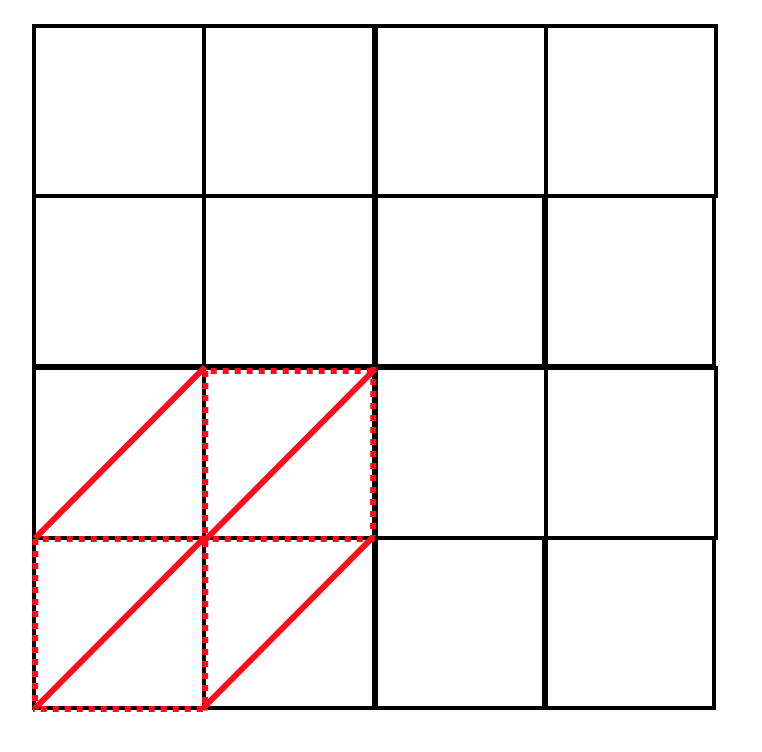
\includegraphics[width=0.5\linewidth]{cellGeneration.png}
  \caption{Cellular Graph generated from Grid}
\end{minipage}%
\pause
\begin{minipage}{.5\textwidth}
  \centering
  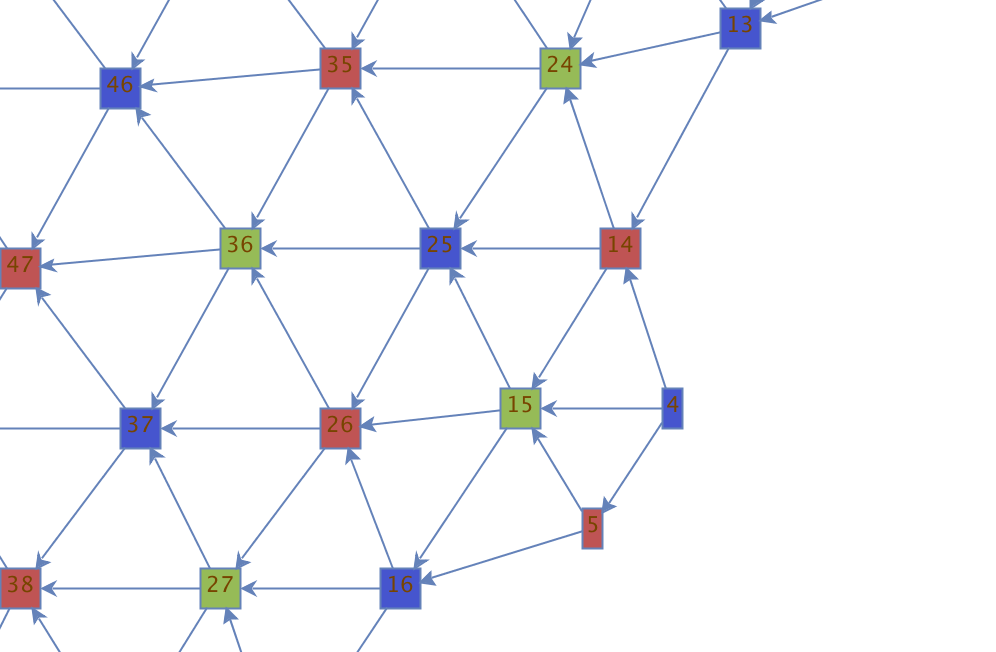
\includegraphics[width=0.65\linewidth]{3colors.png}
  \caption{Part of a colored Cellular Graph}
\end{minipage}
\end{figure}

\scriptsize [1]“Welcome to JGraphT - a free Java Graph Library.” [Online]. Available: http://jgrapht.org/.
\end{frame}



%------------------------------------------------
\begin{frame}{Results and Analysis}

\begin{block}{Running Time Comparison with ILP Solution from GNU}
2 Parameters to evaluate for the time consumption:
\begin{itemize}
\item \textbf{Size} of the Graph
\item \textbf{Nbr of Colors} Available
\end{itemize}
 
\end{block}
\pause
Generation of numerous amount of data \textrightarrow{} Space \& Time limit\\
\pause \textrightarrow{}  Bash Scripts to \textbf{generate}, \textbf{verify}, \textbf{compare} and \textbf{save}\\
\pause \textrightarrow{}  Analysis of the quantitative data in R Studio

% \begin{figure}
% 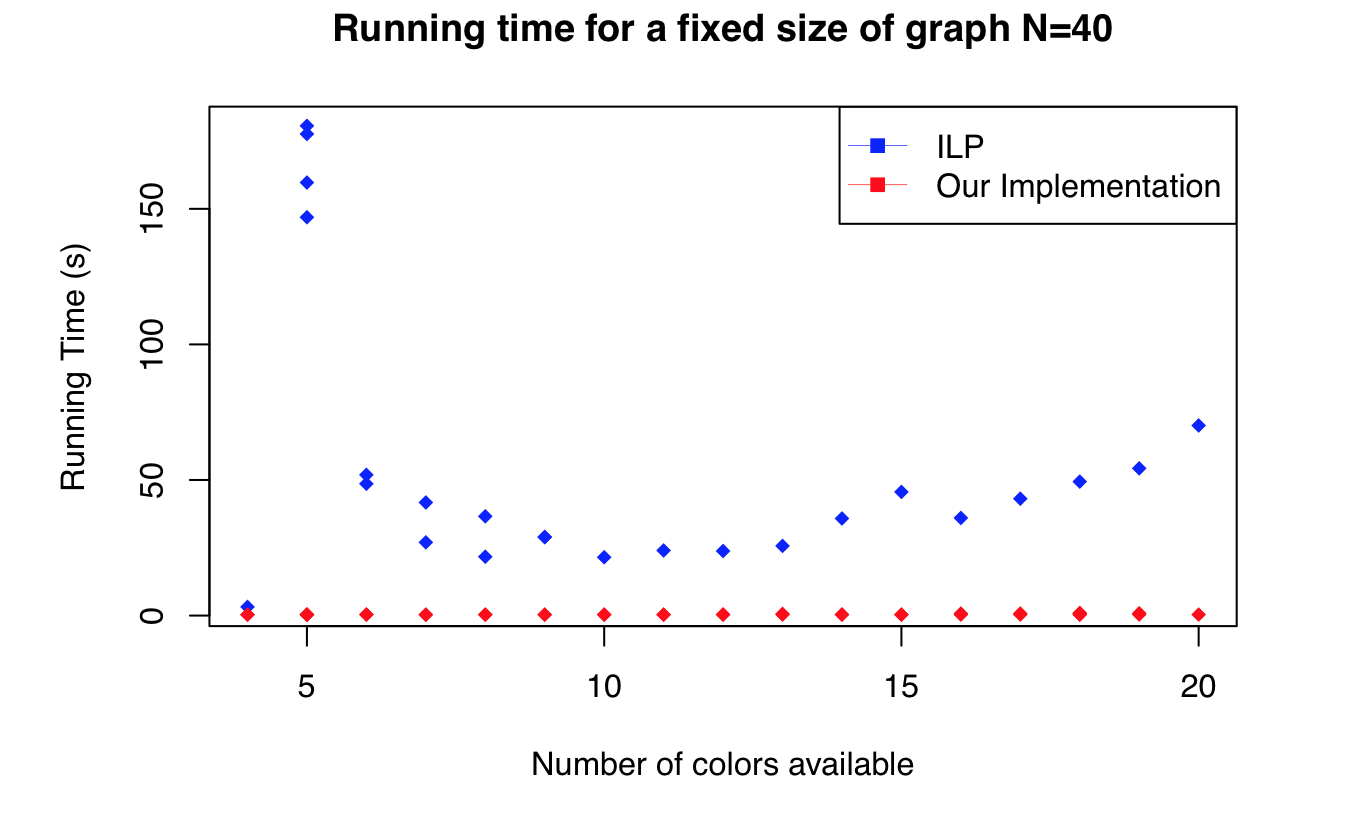
\includegraphics[width=0.8\linewidth]{40SizeRunTime.png}
% \end{figure}

\begin{figure}
\centering
\begin{minipage}{.5\textwidth}
  \centering
  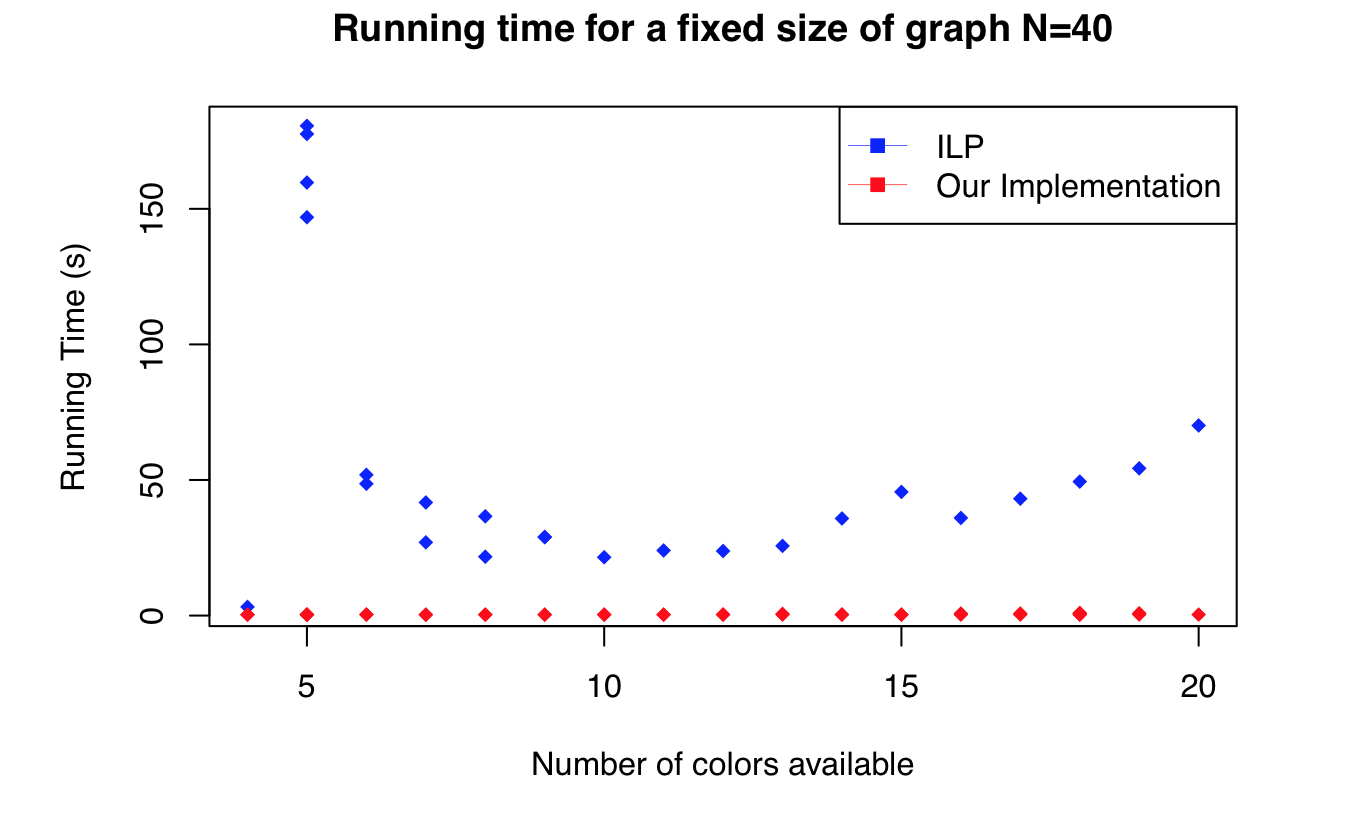
\includegraphics[width=1\linewidth]{40SizeRunTime.png}
  \label{fig:test1}
\end{minipage}%
\begin{minipage}{.5\textwidth}
  \centering
  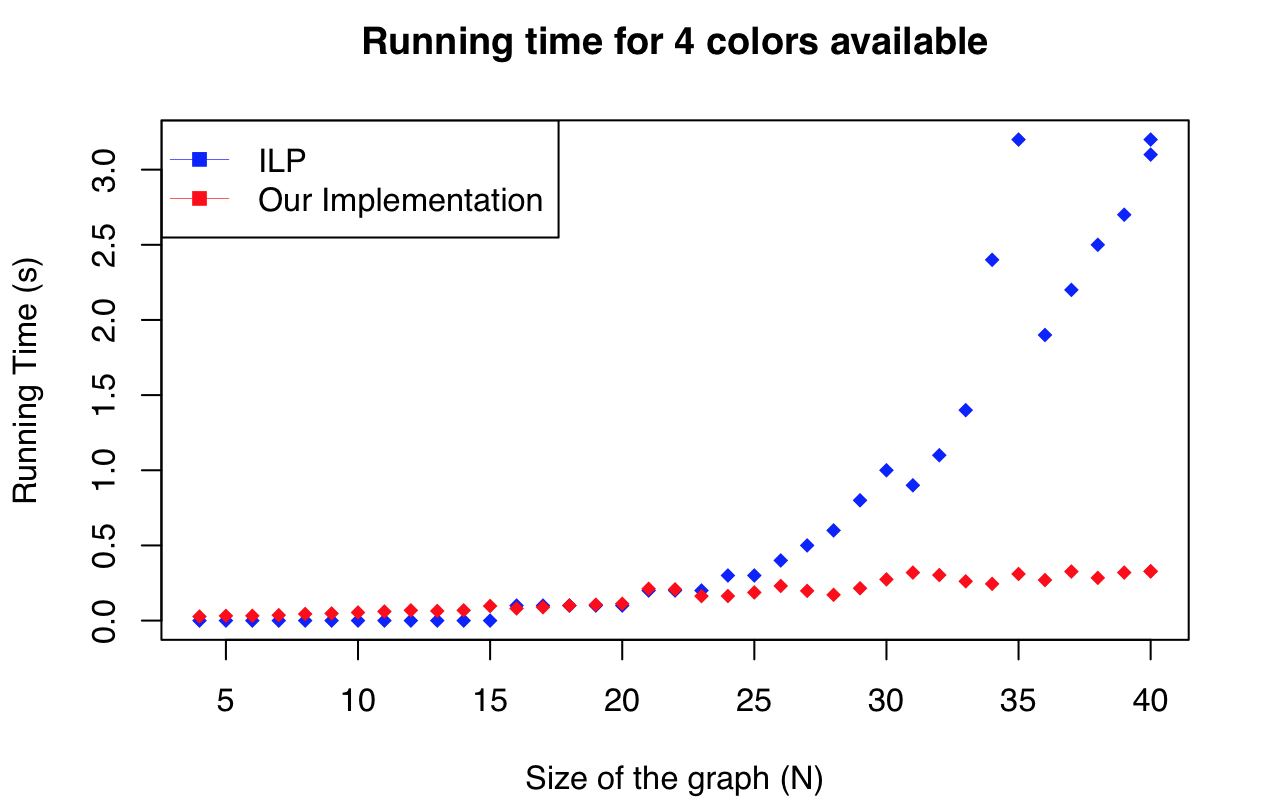
\includegraphics[width=1\linewidth]{4colorsRunTime.png}
  \label{fig:test2}
\end{minipage}
\end{figure}

\vskip 1cm

\end{frame}

%------------------------------------------------
\section{Conclusion}

\begin{frame}{Conclusion}

\begin{block}{}
\begin{itemize}
\item Cellular graph are \textbf{4-choosable} \textrightarrow{} tested
\item When 4 colors available for all Nodes \textrightarrow{} \textbf{3} colors used\\
\textrightarrow{} 1-band buffering cellular graphs are \textbf{3-colorable}
\end{itemize}
 
\end{block}

\vskip 1cm
\pause

\begin{block}{}

\begin{itemize}
\item Running Time (Size, Nbr Available Colors)
\item More \textbf{efficient} than ILP implementation (+ large graph)
\end{itemize}

\end{block}

\end{frame}


%------------------------------------------------
\section{Future Work}

\begin{frame}{Future Work}

\begin{itemize}
  \item Extending the results to $k > 1$.
  \vskip 1cm
  \item Local graph algorithms.
\end{itemize}

\end{frame}

%------------------------------------------------
\section{Questions}

\begin{frame}
\Huge{Thank you for your attention !\\
Do you have any questions?}
\end{frame}




\end{document}
